\documentclass[12pt,a4paper]{article}

\usepackage[top=2.5cm, bottom=2.5cm, left=2.5cm, right=2.5cm]{geometry}
\usepackage[utf8]{inputenc}
\usepackage[T1]{fontenc}
\usepackage{lmodern}
\usepackage{microtype}
\usepackage{graphicx}
\usepackage{booktabs}
\usepackage{tabularx}
\usepackage{hyperref}
\usepackage{xcolor}
\usepackage{listings}
\usepackage{tikz}
\usetikzlibrary{arrows.meta, shapes.geometric, positioning, calc, backgrounds, fit}
\usepackage{parskip}
\usepackage{titlesec}
\usepackage{fancyhdr}
\usepackage{enumitem}
\usepackage{caption}
\usepackage{subcaption}
\usepackage{float}
\usepackage{amsmath}
\usepackage{pifont}  % for \checkmark variant

% ── Page style ────────────────────────────────────────────────────────────────
\pagestyle{fancy}
\fancyhf{}
\lhead{\small Immersive Technologies — A.Y.\ 2024--2025}
\rhead{\small \textit{Action!}}
\cfoot{\thepage}
\renewcommand{\headrulewidth}{0.4pt}

% ── Section headings ──────────────────────────────────────────────────────────
\titleformat{\section}{\large\bfseries}{\thesection.}{0.6em}{}[\vspace{-0.3em}\rule{\linewidth}{0.4pt}]
\titleformat{\subsection}{\normalsize\bfseries}{\thesubsection}{0.5em}{}
\titleformat{\subsubsection}{\normalsize\itshape}{\thesubsubsection}{0.5em}{}

% ── Code listings ─────────────────────────────────────────────────────────────
\lstdefinestyle{csharp}{
  language=[Sharp]C,
  basicstyle=\ttfamily\footnotesize,
  keywordstyle=\color{blue!80!black}\bfseries,
  commentstyle=\color{gray!70},
  stringstyle=\color{red!65!black},
  numberstyle=\tiny\color{gray},
  numbers=left, numbersep=6pt,
  breaklines=true,
  showstringspaces=false,
  frame=single, rulecolor=\color{gray!40},
  tabsize=4,
  captionpos=b
}
\lstset{style=csharp}

% ── Hyperlinks ────────────────────────────────────────────────────────────────
\hypersetup{
  colorlinks=true,
  linkcolor=blue!60!black,
  urlcolor=blue!60!black,
  citecolor=blue!60!black
}

% ── Helpers ───────────────────────────────────────────────────────────────────
\newcommand{\yes}{\ding{51}}   % checkmark
\newcommand{\code}[1]{\texttt{#1}}
\newcommand{\todo}[1]{\textcolor{red!70!black}{\textbf{[TODO: #1]}}}

% ══════════════════════════════════════════════════════════════════════════════
\begin{document}

% ── Title page ────────────────────────────────────────────────────────────────
\begin{titlepage}
  \centering
  \vspace*{1.5cm}

  {\fontsize{42}{50}\bfseries Action!\par}
  \vspace{0.4cm}
  {\large\itshape An Asymmetric Collaborative Virtual Reality Experience\par}

  \vspace{1.2cm}
  \rule{0.6\linewidth}{0.6pt}
  \vspace{1.2cm}

  {\normalsize
    \begin{tabular}{ll}
      \textbf{Mattis Witschi}   & \texttt{mattis.witschi@studenti.unitn.it}   \\
                                 & Matricola:\ 2401922 \\[0.6em]
      \textbf{Lucas Desproges}  & \texttt{lucas.desproges@studenti.unitn.it}  \\
                                 & Matricola:\ \todo{Lucas matricola} \\
    \end{tabular}
  }

  \vspace{1.6cm}
  {\normalsize
    Immersive Technologies \\[0.2em]
    Department of Information Engineering and Computer Science \\[0.2em]
    University of Trento \\[0.5em]
    Academic Year 2024--2025
  }

  \vspace{1.2cm}
  {\small Repository: \texttt{https://github.com/}\todo{repo}\par}
  \vfill
  {\small \today}
\end{titlepage}

% ── Abstract ──────────────────────────────────────────────────────────────────
\section*{Abstract}
\addcontentsline{toc}{section}{Abstract}

\textit{Action!} is an asymmetric collaborative two-player experience developed in Unity~6 using the Ubiq social VR framework and the XR Interaction Toolkit on Meta Quest headsets. The project casts one player as an \textbf{Actor}---physically inhabiting a virtual apartment set, guided step by step by a head-mounted HUD---and the second as a \textbf{Director}, operating from an adjacent control booth where physical levers and push-buttons trigger environmental effects such as lighting changes, weather events, and music playback. Collaboration is enforced through a synchronisation mechanic: the Director must fire the correct effect within a two-second window of the Actor's action; missing the window resets the scene. Communication relies exclusively on Ubiq's integrated voice chat, making verbal coordination the core gameplay loop.

The project was implemented in two phases: a complete desktop prototype---validated across a nine-step scenario---followed by a migration to Meta Quest VR. The desktop phase established the full game logic, Ubiq networking, and scenario state machine. The VR phase introduced XRI-based physical interaction (grab, teleportation, button press), 3D XR-interactable lobby panels, and Ubiq avatar synchronisation. Key engineering challenges included integrating Ubiq's peer-to-peer networking with XRI's grab-ownership model, preventing sticky-hand artefacts when interactors select physical objects, synchronising networked object state across clients, and supporting mixed-platform sessions (PC + Quest).

Informal evaluation with five participants confirmed the appeal of the coordination mechanic and highlighted the need for a richer narrative scenario. Participants appreciated the physical VR interaction and the sense of genuine interdependence between roles. The main limitation identified was the thinness of the current morning-routine scenario; a planned redesign around a magic-show theme would better exploit the Director's capacity to trigger spectacular effects. Lessons learned point toward a cleaner PC-Director / VR-Actor split and earlier mastery of the Ubiq framework as the two highest-impact improvements for future iterations.

\medskip
\noindent\textbf{Keywords:} asymmetric multiplayer, social VR, Ubiq, XR Interaction Toolkit, Unity~6, cooperative games, Meta Quest.

\newpage
\tableofcontents
\newpage

% ══════════════════════════════════════════════════════════════════════════════
\section{Introduction}
\label{sec:intro}

Collaborative virtual reality opens interaction possibilities that differ fundamentally from both single-player VR and traditional screen-based multiplayer: users share a physical-scale space, communicate through embodied avatars, and manipulate a common environment with their hands. Within this broad design space, \emph{asymmetric} experiences---where two players have structurally different roles, tools, and perspectives---remain comparatively under-explored. The most widely known example, \emph{Keep Talking and Nobody Explodes}~\cite{keeptalking2015}, divides players across physical-space boundaries: one wears a VR headset and sees an armed device; the others consult a printed manual and verbally guide the first. The experience derives its tension from information asymmetry and the impossibility of unilateral success.

\textit{Action!} explores a complementary asymmetry grounded in \emph{live theatrical and cinematic production}. One player---the \textbf{Actor}---inhabits the virtual set and executes a scripted sequence of actions. The second---the \textbf{Director}---occupies a separate control booth and must fire the correct environmental effect (a burst of rain, a change of lighting, a music cue) in tight synchrony with the Actor's performance. Neither role can succeed alone; the Actor cannot trigger effects and the Director cannot navigate the set. Success depends entirely on real-time verbal coordination through integrated voice chat.

The project was developed for the \textit{Immersive Technologies} course at the University of Trento (A.Y.\ 2024--2025). Development proceeded in two main phases. First, a complete desktop prototype was built and validated across a nine-step scenario using keyboard-and-mouse input. Second, a VR migration was performed targeting the Meta Quest platform, adapting the Actor's role to full room-scale interaction and introducing Ubiq avatar synchronisation and a multiplayer lobby system.

\medskip
\noindent\textbf{Contributions of this work:}
\begin{itemize}[leftmargin=1.8em, itemsep=2pt]
  \item A design and working prototype of an asymmetric two-player VR experience built on Unity~6, Ubiq, and XRI 3.x.
  \item A nine-step narrative scenario with state-machine-driven synchronisation across networked clients.
  \item A platform-adaptive lobby and role-selection system supporting Quest-to-Quest and PC-to-Quest sessions.
  \item A catalogue of engineering patterns (SafeSelect coroutine, single-rig architecture, mixed-platform detection) for combining Ubiq networking with XRI interaction.
  \item A critical analysis of the challenges encountered and a set of concrete lessons for future asymmetric VR projects.
\end{itemize}

\medskip
The remainder of the report is structured as follows: Section~\ref{sec:related} surveys related work; Section~\ref{sec:design} presents the design and scenario; Section~\ref{sec:impl} details the implementation; Section~\ref{sec:eval} reports the evaluation; Section~\ref{sec:discussion} discusses limitations and future work.

% ══════════════════════════════════════════════════════════════════════════════
\section{Related Work}
\label{sec:related}

\subsection{Asymmetric Multiplayer Games}

Asymmetric game design---where players operate under structurally different rules, information sets, or capabilities---has been identified as a particularly effective driver of communication and social engagement. Depping et al.~\cite{depping2016} showed that tight interdependence between players in cooperative games significantly increases co-presence and enjoyment, especially when each player's capabilities are complementary rather than identical. \textit{Keep Talking and Nobody Explodes}~\cite{keeptalking2015} remains the canonical VR example: the VR player and the manual-reading players share no common information channel except voice, making communication the primary game mechanic. \textit{Action!} extends this paradigm by introducing \emph{temporal} asymmetry: the Director must not merely communicate information but act at precisely the right moment, adding a time-pressure dimension on top of the information gap.

\textit{Among Us}~\cite{innersloth2018} demonstrates that asymmetric roles within a shared environment can sustain rich verbal and social dynamics in relatively simple game contexts. Our work applies analogous logic to a constructive---rather than adversarial---task, where both players succeed or fail together.

\subsection{Social and Collaborative Virtual Reality}

The Ubiq framework~\cite{friston2022}, developed at University College London, provides a Unity-based open-source platform for multi-user VR applications, offering peer-to-peer networking, voice chat, and avatar synchronisation out of the box. Its design explicitly targets flexible, research-oriented social VR prototyping. We adopt Ubiq as the networking backbone of \textit{Action!} and contribute practical experience integrating it with Unity's XR Interaction Toolkit---a combination not well documented in existing tutorials.

Greenwald et al.~\cite{greenwald2017} surveyed collaborative learning applications in social VR and identified shared object manipulation, role differentiation, and voice communication as consistently the most effective engagement drivers. \textit{Action!} integrates all three: the Actor manipulates grabbable objects whose state is synchronised across clients; the two players have structurally distinct roles; and voice is the primary coordination channel.

\subsection{Presence and Physical Interaction in VR}

Slater's framework~\cite{slater2009} identifies \emph{place illusion} (the sense of being physically present in the virtual environment) and \emph{plausibility} (the sense that events are really occurring) as the two dimensions of VR presence that drive realistic behaviour. Physical interaction---grabbing, pressing, and manipulating objects with tracked hands---directly reinforces both. Our implementation leverages XRI's \texttt{XRGrabInteractable} and \texttt{XRSimpleInteractable} for this reason, and the Actor's ability to physically pick up objects, cross doors, and press light switches is an intentional design choice to maximise physical plausibility.

% ══════════════════════════════════════════════════════════════════════════════
\section{Design and Walkthrough}
\label{sec:design}

\subsection{Design Rationale}

The metaphor of \textit{Action!} is borrowed from live television production: the Actor is the performer on set; the Director controls the hidden technical infrastructure that brings the scene to life. This framing justifies the asymmetry naturally---a real actor does not operate the lighting console---and offers a rich vocabulary of future effects (camera cuts, fog machines, pyrotechnics, flying props). The central design question was: \emph{can two players, each equipped with fundamentally different interaction tools, collaborate effectively through voice alone?}

Three principles guide the design:

\begin{enumerate}[leftmargin=1.8em, itemsep=3pt]
  \item \textbf{Embodied interdependence.} Neither player can complete the scenario alone. The Actor triggers actions; the Director triggers effects. Neither step advances without the other where synchronisation is required.
  \item \textbf{Temporal coupling.} A two-second synchronisation window creates time pressure and demands that players predict each other's rhythm, not merely react.
  \item \textbf{Voice as the primary mechanic.} Voice chat is not optional peripheral support---it is the only coordination channel. The quality of the players' communication directly determines their score.
\end{enumerate}

\subsection{Player Roles}

\paragraph{Actor.} The Actor starts inside a furnished virtual apartment and receives a sequential to-do list through a head-mounted HUD. Only the current instruction is visible; the next is revealed only on completion. Locomotion uses VR teleportation (arc ray, left joystick). Objects are grabbed with the grip trigger. The Actor has no control over any environmental effect.

\paragraph{Director.} The Director stands in a control booth adjacent to the set, equipped with a console of push-buttons and toggle levers, each wired to a named effect. A remote-camera monitor displays the Actor's current position, providing spatial awareness without direct line-of-sight. The Director listens to the Actor's voice cues and triggers effects at the correct moment.

\begin{figure}[H]
  \centering
  % ── INSERT SCREENSHOT: Vue cabine réalisateur — boutons, leviers, moniteur avec vue acteur ──
  \fbox{\parbox{0.78\linewidth}{\centering\vspace{2.5cm}
    \textit{[Screenshot: Director's control booth — buttons, levers, remote-camera monitor]}
  \vspace{2.5cm}}}
  \caption{The Director's control booth. Push-buttons (Sound, Weather, Light, Music) and toggle levers (Day/Night) are physically interactable in VR. The remote-camera monitor displays the Actor's real-time position.}
  \label{fig:booth}
\end{figure}

\subsection{Scenario Walkthrough}

The prototype scenario unfolds across nine ordered steps set in a domestic apartment. Table~\ref{tab:scenario} summarises the full sequence.

\begin{table}[H]
  \centering
  \caption{Nine-step prototype scenario. \yes\ = synchronisation required (2\,s window).}
  \label{tab:scenario}
  \small
  \begin{tabularx}{\linewidth}{@{} c X X c @{}}
    \toprule
    \textbf{\#} & \textbf{Actor action} & \textbf{Director effect} & \textbf{Sync} \\
    \midrule
    1 & Wake up (automatic, 2\,s timer) & --- & \\
    2 & Interact with TV & Sound on & \yes \\
    3 & Read the newspaper & Day/Night toggle (dawn) & \\
    4 & Cross main door & --- & \\
    5 & Pick up coffee cup & --- & \\
    6 & Place CD in music box & Music on & \yes \\
    7 & Cross garden door & Weather effect & \\
    8 & Toggle light switch & Light effect & \yes \\
    9 & Lie down in bed & Day/Night toggle (night) & \yes \\
    \bottomrule
  \end{tabularx}
\end{table}

\subsection{Synchronisation Mechanic}

For synchronised steps, the \texttt{SyncChecker} component opens a 2-second window on receipt of the Actor's action message. If the Director triggers the correct named effect within this window the step is marked successful; otherwise the \texttt{ScenarioManager} resets both players' HUDs and scenario state to step~1. The score---visible to both players at session end---is the total number of ``takes'' required to complete all nine steps.

The 2-second window is deliberately generous enough to absorb typical Ubiq peer-to-peer latency (30--80\,ms on a local Wi-Fi network) while still creating meaningful time pressure.

\subsection{Spatial Layout and Visual Design}

The Actor's space is a furnished apartment (living room, hallway, garden access, bedroom). The Director's booth is separated from the set by an opaque wall and uses an industrial aesthetic---metal textures, CRT monitor, toggle switches---to contrast with the warmer domestic environment of the Actor.

\begin{figure}[H]
  \centering
  % ── INSERT SCREENSHOT: Vue acteur dans l'appartement, HUD en haut avec instruction ──
  \fbox{\parbox{0.78\linewidth}{\centering\vspace{2.5cm}
    \textit{[Screenshot: Actor's first-person view — apartment, HUD with current step]}
  \vspace{2.5cm}}}
  \caption{The Actor's perspective. The head-mounted HUD shows the current instruction. Environmental effects triggered by the Director (here: weather) are visible through the window.}
  \label{fig:actor}
\end{figure}

% ══════════════════════════════════════════════════════════════════════════════
\section{Implementation}
\label{sec:impl}

\subsection{Technology Stack}

\begin{center}
\small
\begin{tabular}{@{}ll@{}}
  \toprule
  \textbf{Component} & \textbf{Version / Source} \\
  \midrule
  Unity               & 6000.x (Unity 6) \\
  Render pipeline     & Universal Render Pipeline 17.3 \\
  Networking          & Ubiq (UCL upm branch) \\
  XR SDK              & XR Interaction Toolkit 3.0.7 \\
  OpenXR              & 1.13.0 \\
  XR Hands            & 1.4.0 \\
  Input System        & New Input System 1.18.0 \\
  Target hardware     & Meta Quest 2 / Quest 3 \\
  \bottomrule
\end{tabular}
\end{center}

\subsection{Networking Architecture}

Ubiq provides the networking substrate via its \code{NetworkScene} prefab, which manages peer discovery and message routing through the UCL relay server (\texttt{nexus.cs.ucl.ac.uk:8009}). Three custom \code{NetworkBehaviour} components handle game-specific state:

\begin{itemize}[leftmargin=1.8em, itemsep=2pt]
  \item \code{EffectsSync} --- Director $\to$ all clients; carries the effect name (``Light'', ``Weather'', etc.).
  \item \code{ActorActionsSync} --- Actor $\to$ all clients; carries the interacted object name.
  \item \code{NetworkObjectState} --- per pickup object; synchronises \code{SetActive(false)} when collected.
\end{itemize}

\begin{figure}[H]
\centering
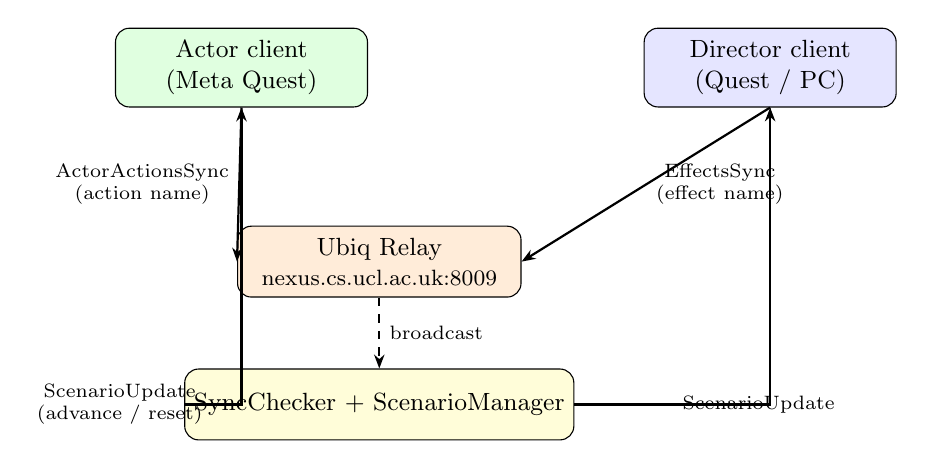
\begin{tikzpicture}[
  node distance = 1.0cm and 2.5cm,
  client/.style = {rectangle, draw, rounded corners=5pt, minimum width=3.2cm,
                   minimum height=1.0cm, align=center, font=\small},
  relay/.style  = {rectangle, draw, fill=orange!15, rounded corners=5pt,
                   minimum width=3.6cm, minimum height=0.9cm, align=center, font=\small},
  lbl/.style    = {font=\scriptsize, align=center},
  arr/.style    = {-{Stealth[length=5pt]}, thick}
]
  \node[client, fill=green!12]  (A) {Actor client\\(Meta Quest)};
  \node[client, fill=blue!10, right=3.5cm of A] (D) {Director client\\(Quest / PC)};
  \node[relay, below=1.5cm of A, xshift=1.75cm] (R)
        {Ubiq Relay\\{\footnotesize nexus.cs.ucl.ac.uk:8009}};
  \node[relay, fill=yellow!15, below=0.9cm of R] (S)
        {SyncChecker + ScenarioManager};

  \draw[arr] (A.south) -- node[lbl,left]{ActorActionsSync\\(action name)} (R.west);
  \draw[arr] (D.south) -- node[lbl,right]{EffectsSync\\(effect name)} (R.east);
  \draw[arr, dashed] (R) -- node[lbl,right]{broadcast} (S);
  \draw[arr] (S.west) -| node[lbl,left,pos=0.25]{ScenarioUpdate\\(advance / reset)} (A.south);
  \draw[arr] (S.east) -| node[lbl,right,pos=0.25]{ScenarioUpdate} (D.south);
\end{tikzpicture}
\caption{Networking architecture. All inter-client messages are routed through the Ubiq relay. \code{SyncChecker} validates timing and drives \code{ScenarioManager} on every client simultaneously.}
\label{fig:network}
\end{figure}

Player avatar transforms are streamed by Ubiq's built-in \code{HeadAndHandsAvatarInputXRI} component, which is enabled on the XR rig after role selection.

\subsection{Lobby and Role-Selection System}

A critical sequencing requirement is that both players must join the same Ubiq room \emph{before} selecting a role, preventing a situation where one player picks ``Actor'' before the other has even connected.

\begin{figure}[H]
\centering
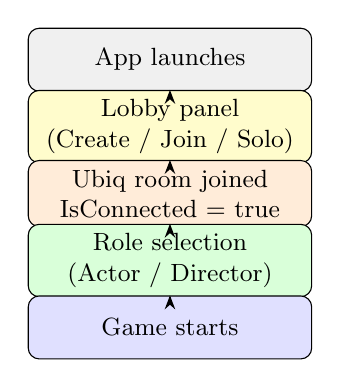
\begin{tikzpicture}[
  box/.style={rectangle, draw, rounded corners=4pt, minimum width=3.6cm,
              minimum height=0.8cm, align=center, font=\small},
  arr/.style={-{Stealth[length=5pt]}, thick},
  node distance=0.85cm
]
  \node[box, fill=gray!12]   (L) {App launches};
  \node[box, fill=yellow!20, below of=L] (P) {Lobby panel\\(Create / Join / Solo)};
  \node[box, fill=orange!15, below of=P] (U) {Ubiq room joined\\{\small IsConnected = true}};
  \node[box, fill=green!15,  below of=U] (R) {Role selection\\(Actor / Director)};
  \node[box, fill=blue!12,   below of=R] (G) {Game starts};
  \draw[arr] (L)--(P); \draw[arr] (P)--(U); \draw[arr] (U)--(R); \draw[arr] (R)--(G);
\end{tikzpicture}
\caption{Session startup flow. The role-selection UI is gated behind \code{UbiqSetup.IsConnected}.}
\label{fig:flow}
\end{figure}

The lobby is implemented in \code{LobbyConnectionPanel}. On desktop it renders a centred \code{OnGUI} overlay. On Meta Quest it procedurally generates three \code{XRSimpleInteractable} cubes (\textsc{Create}, \textsc{Join}, \textsc{Solo}) facing the camera; selecting \textsc{Join} opens a \code{TouchScreenKeyboard} for entering the room code. Platform detection is centralised in \code{XRCheck.IsVR()}, which returns \code{true} unconditionally on Android and queries \code{XRSettings.isDeviceActive} otherwise, resolving an earlier bug where PC builds incorrectly rendered the VR lobby panel.

\begin{figure}[H]
  \centering
  \begin{subfigure}[b]{0.47\linewidth}
    % ── INSERT SCREENSHOT: Panneau OnGUI desktop (créer/rejoindre) ──
    \fbox{\parbox{\linewidth}{\centering\vspace{2cm}
      \textit{[Screenshot: desktop OnGUI\\lobby panel]}
    \vspace{2cm}}}
    \caption{Desktop OnGUI overlay.}
  \end{subfigure}
  \hfill
  \begin{subfigure}[b]{0.47\linewidth}
    % ── INSERT SCREENSHOT: Cubes XR lobby VR (vert/bleu/jaune) ──
    \fbox{\parbox{\linewidth}{\centering\vspace{2cm}
      \textit{[Screenshot: VR lobby cubes\\(Create / Join / Solo)]}
    \vspace{2cm}}}
    \caption{VR 3D-cube lobby panel.}
  \end{subfigure}
  \caption{The lobby connection panel adapts to platform: \code{OnGUI} on desktop, \code{XRSimpleInteractable} cubes in VR.}
  \label{fig:lobby}
\end{figure}

After both players join, role-selection cubes (green = Actor, blue = Director) appear via \code{VRRoleMenu}. On desktop, F1/F2 keyboard shortcuts serve the same purpose.

\subsection{VR Interaction Patterns}

\subsubsection{Director's Console: Sticky-Hand Fix}
Each button and lever in the control booth carries an \code{XRSimpleInteractable}. The custom \code{XRDirectorInteractor} calls the underlying \code{InteractableButton.Press()} or \code{Lever.Toggle()} method on selection, then immediately starts a \code{ReleaseNextFrame} coroutine that force-exits the selection two frames later via \code{XRInteractionManager.SelectExit()}. Without this, the controller hand ``sticks'' to the button because XRI expects the interactable to remain selected until the player physically releases the trigger.

\subsubsection{Actor's Grab Objects: Collider Conflict Fix}
Pickable objects (coffee cup, CD) use \code{XRGrabInteractable}. The desktop prototype's \code{HoldableItem.Interact()} method disabled all object colliders on pickup---breaking XRI's grab detection. The fix: add an early return when the \code{ActorController} argument is \code{null} (the VR code path passes \code{null} since no desktop actor is active), leaving XRI to manage the grab lifecycle entirely.

\subsubsection{Music Box CD Placement}
The music box detects the CD entering its trigger zone via \code{OnTriggerEnter}. Because XRI retains grab ownership until the player releases the trigger, a \code{ReleaseAndPlace} coroutine force-exits the grab, waits two frames, then calls \code{PlaceCD()}.

\subsubsection{Single XR-Rig Architecture}
A key architectural decision was to maintain \emph{one} active \code{XROrigin} rather than switching between an Actor rig and a Director rig via \code{SetActive}. Disabling an active XR Origin while OpenXR is running causes driver crashes in Unity~6. Instead, the single rig (\code{Player\_Actor\_XR}) is teleported to the appropriate spawn point after role selection, and \code{ActorControllerXR} or \code{DirectorControllerXR} is enabled/disabled in place.

\begin{figure}[H]
  \centering
  \begin{subfigure}[b]{0.47\linewidth}
    % ── INSERT SCREENSHOT: Main droite VR saisissant le CD ──
    \fbox{\parbox{\linewidth}{\centering\vspace{2.2cm}
      \textit{[Screenshot: VR hand\\grabbing the CD]}
    \vspace{2.2cm}}}
    \caption{Actor grabbing the CD.}
  \end{subfigure}
  \hfill
  \begin{subfigure}[b]{0.47\linewidth}
    % ── INSERT SCREENSHOT: Main VR appuyant sur un bouton de la cabine réalisateur ──
    \fbox{\parbox{\linewidth}{\centering\vspace{2.2cm}
      \textit{[Screenshot: VR hand pressing\\a Director console button]}
    \vspace{2.2cm}}}
    \caption{Director pressing a button.}
  \end{subfigure}
  \caption{Physical VR interaction. Both roles use the XR Interaction Toolkit with custom force-release coroutines to prevent sticky-hand artefacts.}
  \label{fig:xri}
\end{figure}

\subsection{Voice Chat and Avatars}
Ubiq's built-in \code{VoipPeer} / \code{VoipSpeakerOutput} pipeline provides voice chat without additional configuration when using the standard \code{NetworkScene} prefab. Avatars (floating head + two hands) are streamed via \code{HeadAndHandsAvatarInputXRI}, enabled after role selection so each player sees the other's avatar move in real time.

% ══════════════════════════════════════════════════════════════════════════════
\section{Evaluation}
\label{sec:eval}

\subsection{Method}
We conducted an informal qualitative evaluation with five participants: the two developers and three external users (fellow students). Each session lasted approximately 20~minutes and comprised one full playthrough of the nine-step scenario followed by an open discussion. No standardised questionnaire was used; observations and verbal feedback were recorded during and after each session. Testing was conducted in desktop mode (local network, keyboard-and-mouse for both players) to validate the complete scenario, supplemented by partial VR testing with one Meta Quest headset.

\subsection{Results}

\paragraph{Engagement and coordination.}
All five participants found the interdependence mechanic compelling. The structural dependency---Actor cannot advance without the Director; Director cannot act without the Actor's signal---naturally prompted rich verbal communication. Participants spontaneously developed call-and-response conventions (\textit{``Ready for the light switch\ldots''} / \textit{``On it!''}) within the first two minutes of play. No tutorialisation was needed to motivate voice use.

\paragraph{Physical interaction.}
The physical aspects of VR (grabbing the CD, pressing buttons with a virtual hand, teleporting across rooms) were consistently cited as more satisfying than their mouse-click equivalents. One participant noted that walking into a new room and pressing a physical switch felt \textit{``way more real than clicking a button on screen.''} The Director's remote-camera monitor---showing the Actor's position in real time---was praised as essential: without it the Director felt ``blind.''

\paragraph{Narrative and scenario depth.}
The main criticism was the thinness of the scenario. The morning-routine setting felt arbitrary, and participants struggled to build emotional investment. One participant summarised: \textit{``The principle of the game is interesting---it's a real coordination game---but it needs to be part of a bigger story.''} The individual effects (rain, music, lights) were perceived as technically impressive but insufficiently integrated into a coherent narrative arc.

\paragraph{Technical friction.}
The lobby room-joining flow was identified as a UX friction point: participants found the manual entry of a room code unintuitive and occasional Wi-Fi-related connection drops disrupted sessions. The VR migration was only partially stable during the evaluation period; full Quest-to-Quest sessions with both players in VR were not reliably achievable.

\subsection{Summary}
The core asymmetric mechanic and the synchronisation system were validated as engaging and novel. The technical infrastructure proved sufficient to run coherent nine-step desktop sessions. The main gaps between prototype and polished product are narrative design, lobby UX, and VR network stability.

% ══════════════════════════════════════════════════════════════════════════════
\section{Discussion and Conclusions}
\label{sec:discussion}

\subsection{Lessons Learned}

\paragraph{Build for VR from the start.}
Our two-phase approach (desktop first, then VR migration) introduced significant rework. Design decisions that were natural for desktop---cursor-based UI, collision-driven pickup, per-platform active-player flags---became obstacles in VR. In retrospect, building directly for VR even with placeholder interactions would have saved debugging time and produced a more coherent interaction model.

\paragraph{Master the networking layer before the game layer.}
Ubiq's peer-to-peer model is powerful but its edge cases---reconnection, mid-session state sync, interplay with XRI's ownership model---are poorly documented. We spent a disproportionate share of total development time on networking bugs (double-subscription to Ubiq events, timing races between \code{OnJoinedRoom} and \code{RoleSelector}, VoipSpeechIndicator null-reference exceptions). Investing in a small standalone Ubiq + XRI testbed before the main project would have paid dividends.

\paragraph{Separate platforms by role.}
Both evaluation feedback and implementation experience converge on the same conclusion: the natural platform split is \textbf{Director on PC, Actor in VR}. The Director benefits from a large screen, a mouse-driven 2D control panel, and keyboard shortcuts. The Actor benefits from full physical immersion. Attempting to make both roles VR-compatible simultaneously added engineering complexity without proportional design benefit.

\subsection{Future Work}

\paragraph{Magic-show scenario.}
The most impactful redesign would reframe the scenario around a \textbf{stage magician} performance: the Actor plays the magician; the Director operates hidden stage machinery---trap doors, smoke effects, levitating props, lighting rigs---that makes the illusions succeed. This theme provides a natural justification for spectacular synchronised effects, a coherent narrative arc, and an intuitive understanding of each role's function.

\paragraph{PC Director interface.}
A dedicated 2D control-room UI for the Director (full-screen on a PC monitor rather than a VR scene repurposed for desktop) would remove the single-rig complexity and allow richer effect-management interfaces (multiple simultaneous effects, cue timelines).

\paragraph{Progressive difficulty.}
Reducing the synchronisation window from 2~s to 1~s (or less) as the scenario progresses would create a genuine difficulty curve and reward experienced teams.

\paragraph{Lobby robustness.}
Automatic reconnection, persistent room codes, and a QR-code join flow would substantially reduce session-setup friction.

\subsection{Conclusions}

\textit{Action!} demonstrates that the Director-Actor metaphor translates effectively into an engaging VR experience. The synchronisation mechanic creates genuine temporal pressure and motivates rich verbal coordination without requiring any explicit tutorial. The prototype validates the core concept; the infrastructure (Ubiq networking, XRI interaction, Ubiq voice chat) is in place for a fully polished product. The primary next step is elevating the narrative scenario to match the technical capability already built.

% ══════════════════════════════════════════════════════════════════════════════
\newpage
\section*{Group Contribution Statement}
\addcontentsline{toc}{section}{Group Contribution Statement}

Both team members contributed to all phases of the project---design, implementation, testing, and documentation---in equal measure. Development was conducted collaboratively through paired work sessions and frequent synchronisation; no formal division of tasks by domain was established.

\begin{center}
\begin{tabular}{@{}lll@{}}
  \toprule
  \textbf{Member} & \textbf{Email} & \textbf{Contribution} \\
  \midrule
  Mattis Witschi  & mattis.witschi@studenti.unitn.it  & 50\% \\
  Lucas Desproges & lucas.desproges@studenti.unitn.it & 50\% \\
  \bottomrule
\end{tabular}
\end{center}

Both members certify that the work presented in this report is original and that all external sources are properly cited.

% ══════════════════════════════════════════════════════════════════════════════
\newpage
\bibliographystyle{plain}
\begin{thebibliography}{9}

\bibitem{keeptalking2015}
Steel Crate Games.
\newblock \textit{Keep Talking and Nobody Explodes}.
\newblock Video game, 2015.
\newblock \url{https://www.keeptalkinggame.com/}

\bibitem{depping2016}
A.\,E.~Depping, C.~Johanson, and R.\,L.~Mandryk.
\newblock Cooperation and interdependence: How multiplayer games engage players.
\newblock In \textit{Proc.\ Annual Symposium on Computer-Human Interaction in Play (CHI PLAY)}, pages 455--467. ACM, 2016.

\bibitem{innersloth2018}
Innersloth.
\newblock \textit{Among Us}.
\newblock Video game, 2018.
\newblock \url{https://www.innersloth.com/games/among-us/}

\bibitem{friston2022}
S.~Friston, B.~Congdon, D.~Swapp, L.~Eckert, K.~Akamine, W.~Ryan,
G.~Wilson, C.~Vertigan, and A.~Steed.
\newblock Ubiq: A system to build flexible social virtual reality experiences.
\newblock In \textit{Proc.\ ACM International Conference on Interactive Media Experiences (IMX)}, pages 202--212. ACM, 2022.

\bibitem{greenwald2017}
S.\,W.~Greenwald, Z.~Corning, and P.~Maes.
\newblock Multi-user framework for collaboration and co-presence in virtual reality.
\newblock In \textit{Proc.\ IEEE VR Workshop on Collaborative and Telepresence-Based VR}, 2017.

\bibitem{slater2009}
M.~Slater.
\newblock Place illusion and plausibility can lead to realistic behaviour in
  immersive virtual environments.
\newblock \textit{Philosophical Transactions of the Royal Society B}, 364(1535):3549--3557, 2009.

\bibitem{unity_xri}
Unity Technologies.
\newblock \textit{XR Interaction Toolkit — Documentation}, version 3.0, 2024.
\newblock \url{https://docs.unity3d.com/Packages/com.unity.xr.interaction.toolkit@3.0/manual/}

\end{thebibliography}

% ══════════════════════════════════════════════════════════════════════════════
\newpage
\section*{Code Appendix}
\addcontentsline{toc}{section}{Code Appendix}

Full source: \texttt{https://github.com/}\todo{repo}\texttt{/VRMirrorWorld}

\subsection*{A — Platform Detection}

\begin{lstlisting}[caption={XRCheck.cs — centralised VR/desktop detection.}]
public static class XRCheck
{
    public static bool IsVR()
    {
#if UNITY_ANDROID
        return true;                   // Meta Quest always VR
#else
        return XRSettings.isDeviceActive;  // PC: only if headset active
#endif
    }
}
\end{lstlisting}

\subsection*{B — SafeSelect: Force-Release XRI Interactor}

\begin{lstlisting}[caption={SafeSelect coroutine (LobbyConnectionPanel / VRRoleMenu).}]
private IEnumerator SafeSelect(XRSimpleInteractable cube, Action action)
{
    var manager = FindFirstObjectByType<XRInteractionManager>();
    if (manager != null)
    {
        var selecting = new List<IXRSelectInteractor>(cube.interactorsSelecting);
        foreach (var i in selecting)
            manager.SelectExit(i, cube);
    }
    cube.enabled = false;
    yield return null;
    yield return null;   // wait 2 frames for XRI to finalise the exit event
    action();
}
\end{lstlisting}

\subsection*{C — Director Sticky-Hand Fix}

\begin{lstlisting}[caption={XRDirectorInteractor.cs — force-release after button/lever press.}]
private IEnumerator ReleaseNextFrame(XRBaseInteractable interactable)
{
    if (interactable == null) yield break;
    yield return null;
    yield return null;
    var manager = FindFirstObjectByType<XRInteractionManager>();
    if (manager == null) yield break;
    var selecting = new List<IXRSelectInteractor>(interactable.interactorsSelecting);
    foreach (var i in selecting)
        manager.SelectExit(i, interactable);
}
\end{lstlisting}

\subsection*{D — HoldableItem VR Compatibility}

\begin{lstlisting}[caption={HoldableItem.cs — early return prevents collider conflict with XRGrabInteractable.}]
public void Interact(ActorController actor)
{
    // VR: XRGrabInteractable owns the lifecycle; touching colliders breaks it
    if (actor == null) return;
    if (m_isHeld) return;
    // ... desktop-only grab logic
}
\end{lstlisting}

\subsection*{E — Music Box CD Placement in VR}

\begin{lstlisting}[caption={MusicBoxController.cs — force-release grab before placing the CD.}]
private void OnTriggerEnter(Collider other)
{
    if (m_cdInserted) return;
    var cd   = other.GetComponent<HoldableItem>();
    var grab = other.GetComponent<XRGrabInteractable>();
    if (cd != null)
        StartCoroutine(ReleaseAndPlace(cd, grab));
}

private IEnumerator ReleaseAndPlace(HoldableItem cd, XRGrabInteractable grab)
{
    if (grab != null)
    {
        var manager = FindFirstObjectByType<XRInteractionManager>();
        if (manager != null)
            foreach (var i in new List<IXRSelectInteractor>(grab.interactorsSelecting))
                manager.SelectExit(i, grab);
        yield return null;
        yield return null;
    }
    PlaceCD(cd);
}
\end{lstlisting}

\subsection*{F — Lobby Connection Panel (OnGUI excerpt)}

\begin{lstlisting}[caption={LobbyConnectionPanel.cs — desktop OnGUI overlay (shown until Ubiq connected).}]
private void OnGUI()
{
    if (XRCheck.IsVR()) return;
    if (m_ubiqSetup == null || m_ubiqSetup.IsConnected) return;

    float w = 460f, h = 290f;
    float x = (Screen.width  - w) / 2f;
    float y = (Screen.height - h) / 2f;

    GUI.Box(new Rect(x, y, w, h), "");
    if (GUI.Button(new Rect(x+30, y+58, w-60, 42), "CREATE ROOM (Host)"))
        m_ubiqSetup.CreateRoom();

    m_joinCode = GUI.TextField(new Rect(x+135, y+141, 195, 28), m_joinCode);
    if (GUI.Button(new Rect(x+340, y+140, 90, 30), "Join"))
        m_ubiqSetup.JoinRoom(m_joinCode);
}
\end{lstlisting}

\end{document}
